\chapter{Application Design}\label{chapter::decentralizedapps}

\section{Introduction}
	An Application software or \textit{app} is a computer program designed to perform a specific set of tasks or actions for the end user. There are countless number of applications in use today and the majority of them are web applications following a centralized client-server model\cite{raval2016decentralized}.
	
	\begin{figure}[h]
		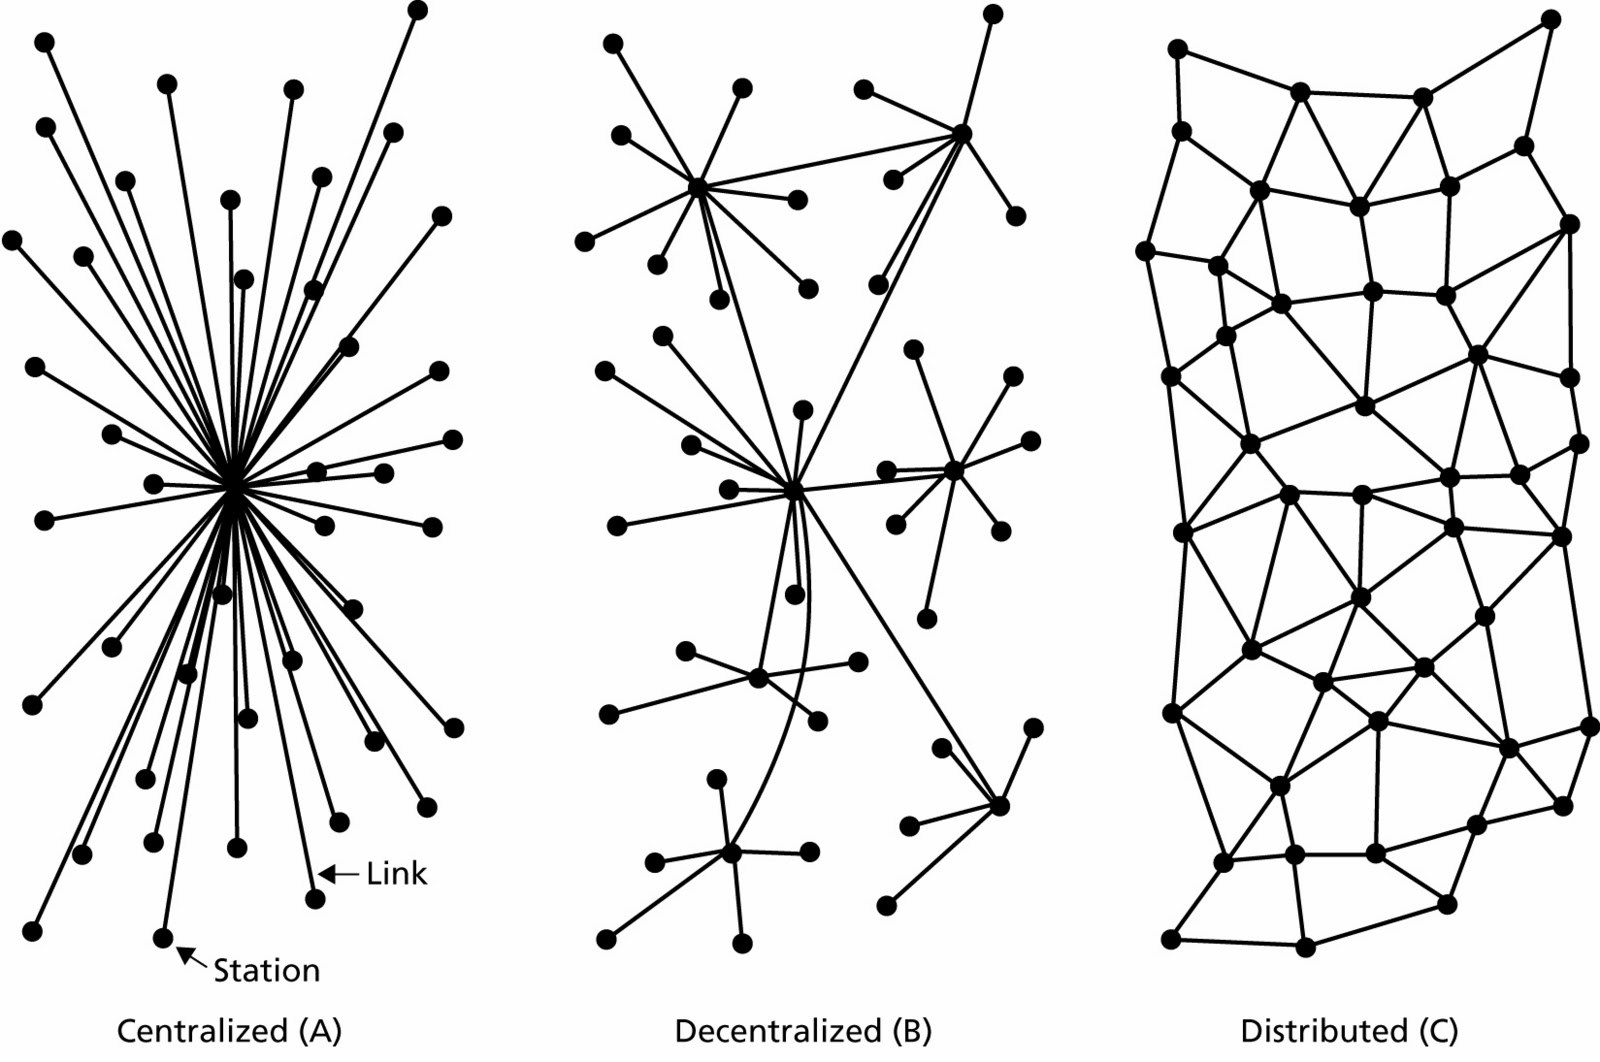
\includegraphics[width=\linewidth]{figures/network-models}
		\caption{\label{fig:applications} The three way of modeling web applications}
	\end{figure}
	
	Figure~\ref{fig:applications} shows a visual representation of three different ways of modeling web applications\cite{baran1964distributed}. Here, \textit{Centralized} and \textit{Decentralized} refers to level of control, while \textit{Distributed} refers to differences of location. Both centralized and decentralized systems can be distributed as well.
	
	\subsection{Centralized}
	It's currently the widespread way of building software applications. In this model a central server control the flow of information and governs the operation of individual units. Since the control is centralized, these types of systems suffer from single point of failure risk.
	
	\subsection{Distributed}
	In a Distributed model, the control still resides with a central server, however, the computation is spread across multiple nodes or servers.
	
	\subsection{Decentralized}
	In a Decentralized model, there is no central point of control as it's spread across all the servers running the application. Applications built using this model don't have a single point of failure and are inherently fault tolerant.

\section{Enabling Technologies}
	The document \textit{Information Management: A Proposal\cite{berners1989information}} written by \textit{Sir Tim Berners-Lee\footnote{\url{https://www.w3.org/People/Berners-Lee/}}} conceived the ideas for what would become the WorldWideWeb. It's main goal was to enable information exchange between computers in an accessible way at CERN\footnote{\url{https://home.cern/}}.
	
	HTML\footnote{\url{https://developer.mozilla.org/en-US/docs/Web/HTML}}, URI\footnote{\url{https://tools.ietf.org/html/rfc3986}} and HTTP\footnote{\url{https://tools.ietf.org/html/rfc2616}} were the fundamental technologies that defined the foundation of the Web. HTTP connected every computer on the planet with a common protocol. The HTTP protocol guidelines defined a set of trusted servers that translated a web address into a server address. Furthermore, HTTPS\footnote{\url{https://tools.ietf.org/html/rfc2818}} added another layer of trusted servers and certificate authorities. People would host personal servers for others to connect to, and everyone owned their data\cite{raval2016decentralized}. As the Web evolved, applications servers\footnote{\url{https://en.wikipedia.org/wiki/Application_server}} became the common way of interactive with the Web and the centralized model of data ownership as we know it today was born\cite{raval2016decentralized}. It was conceptually and programmatically easier to maintain an application server and profit from user's data that utilize it.
	
	Blockchain is the primary technology that enables the creation of applications with a decentralized model of data ownership. It puts the users of an application in control of their data thereby enabling a more open Web, as it was originally intended\footnote{\url{https://webfoundation.org/about/vision/history-of-the-web/}}.
	
	The blockchain helped solve the Byzantine Generals Problem\cite{lamport1982byzantine}. This problem describes a situation where all participating nodes in a distributed network must agree upon every message that is being transmitted between nodes, but where some of the nodes are corrupt and disseminating false information or are unreliable. This agreement is called as \textbf{consensus}. With Bitcoin\cite{nakamoto2008bitcoin}, decentralized consensus became possible. Agreement is achieved in the Bitcoin network by way of \textit{proof-of-work\footnote{\url{https://en.bitcoin.it/wiki/Proof_of_work}}} consensus mechanism which is resistant to Sybil Attack\cite{douceur2002sybil}. Proof-of work is both computationally and energy expensive; other consensus mechanism such as \textit{proof-of-stake\footnote{\url{https://en.bitcoin.it/wiki/Proof_of_Stake}}} relies on stake in the system instead of computational power.
	
\section{Concepts}
	There are five concepts in a web application that have traditionally been implemented in way that puts control with a centralized entity: data, identity, value, computing and bandwidth\cite{raval2016decentralized}. Each of these require trust in a 3rd party - a trust which can be betrayed. Recent advancements in distributed-system technology can put users in control of these things. Below sections describes each concept in detail and shows how one can build applications in a way such that centralized control is not required.

\section{Data}
	Data is the most important concept in any web application. First, let's look at how traditional web applications interact with data. Whenever, a user logs into an application, the application connects to a remote server and sends the authentication details. These details lets the server know which user is interacting with the application. Once authenticated, the user data is fetched from the remote storage and displayed to the user. All complex computations and data storage occurs on dedicated servers maintained in the cloud.
		
	\begin{figure}[h]
		\centering
		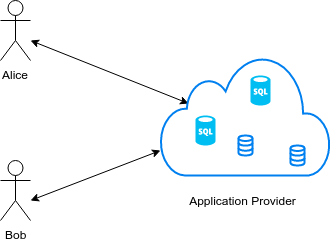
\includegraphics[width=200pt, height=150pt]{figures/traditional-app}
		\caption{\label{fig:traditional-app} How traditional web applications work}
	\end{figure}
		
	Figure~\ref{fig:traditional-app} shows how users interact with a traditional web application. Whenever, Alice wants to interact with Bob, she sends a message to the application server which then delivers the message to Bob. There is no direct path between Alice and Bob. This results in centralization where the provider acts as an intermediary between Alice and Bob's interaction; effectively governing how data is stored and shared among them.
		
	This model of application interaction requires that we trust the providers with out data and hope that they won't misuse or sell our data without our permission. Since revelations by Edward Snowden\cite{greenwald2014no}, we now know that trust can, has and will be broken as long as we entrust our data to a central entity\cite{raval2016decentralized}. Centralized stores of data also serve as a tool for surveillance, allowing big entities to monitor our internet behaviour without our knowledge. Cloud providers, despite having a distributed backend, are centrally owned.
		
	Additionally, as we move from a labor-based economy to an information-based economy, data will become the primary form of value. Therefore, its important that we not only possess our data, but own it as the world evolves. An ideal solution that enables this should provide a way of storing data in a decentralized way that is robust and as trustless as possible\cite{raval2016decentralized}.
	
	\subsection{Storing Data Directly in a Blockchain}
		This method does solves the decentralization of data as everyone who has copy of the Blockchain is storing the data but cannot alter it. The data can be encrypted such that it can only be accessed by someone having the private key. However, Blockchains were not meant for storing large amounts of data. It was designed for storing simple transactional logs, as its evident from looking at the Bitcoin Blockchain where individual records are in bytes\footnote{\url{https://en.bitcoin.it/wiki/Transaction}} and therefore cannot hold much data. Moreover, the Blockchain architecture implies that each node in the network must store a complete copy of the Blockchain. Therefore, storing a significant amount of data on a Blockchain is both expensive and impractical.
		
	\subsection{Storing Data in a Distributed Hash Table}
		DHTs ensure data resiliency by enabling easy distribution and indexing of data. Early peer-to-peer (P2P) filesharing applications like KaZaA\cite{good2003usability}, Napster\cite{ku2002creative} and Gnutella\cite{ripeanu2002mapping} used their own versions of DHTs with a varying degree of decentralization. Some had centralized trackers to monitor the movement of data, while some had central sources from which all data must pass, leaving them with single point of failure\cite{raval2016decentralized}.
		
		BitTorrent\cite{cohen2008bittorrent} was the first protocol to popularize DHT for sharing of large files. As of 2013, BitTorrent has 15–27 million concurrent users at any given time\cite{wang2013measuring}. The BitTorrent Mainline DHT serves as a decentralized data store with centralized trackers to monitor the network. It uses a tit-for-tat strategy between seeders and leechers to maximize the bandwidth of data distribution. This makes the BitTorrent protocol the de facto method for transfer of large datasets over the web. However, using BitTorrent as a data store is not feasible as there is no incentives for nodes to store a data leading to \textit{data impermanence}.
		
		Along with the decentralized storage capabilities of DHT and the speed of BitTorrent's protocol, we also want data permanence. Therefore, its necessary to incentivize the nodes storing the data in some way. Moreover, we also need to ensure that the links to the data don't die, an idea which was first proposed in Project Xanadu\cite{rayward1994visions}.
		
		\subsubsection{InterPlanetary File System (IPFS)} 
			IPFS\cite{benet2014ipfs} is a peer-to-peer file transfer protocol that implements these features, enabling a more permanent, decentralized Web, where links don't die and no single entity controls the data. It achieves this by combining previous peer-to-peer technologies such as DHT, BitTorrent and Git\cite{loeliger2012version}. Data in the IPFS network is modeled as a \textit{merkleDAG\footnote{Similar to a Merkle tree data structure, however, they do not need to be balanced and it's non-leaf nodes can contain some data.}}, a simple data structure that can be conceptualized as a series of nodes connected to each other\cite{raval2016decentralized}. This makes IPFS a \textit{content-addressed\footnote{A content-addressed storage is way to store information such that it can retrieved based on its content and not its location.}} system allowing efficient data lookup and retrieval as it doesn't rely on a single server to access the data.
		
			\begin{figure}[h]
				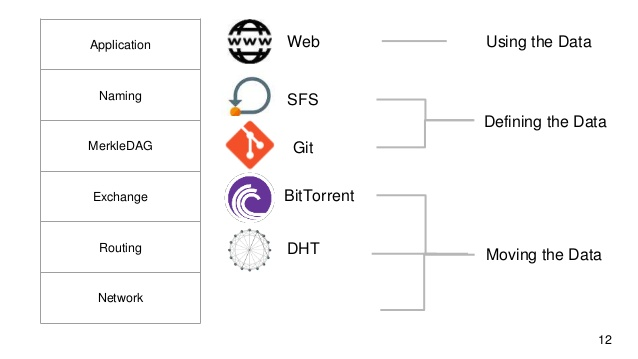
\includegraphics[width=\linewidth]{figures/ipfs-stack}
				\caption{\label{fig:ipfs-stack} IPFS Stack}
			\end{figure}
		
			Filecoin\cite{benet2018filecoin}, a \textit{decentralized storage network}, combines IPFS (shown in Figure~\ref{fig:ipfs-stack}\footnote{Adopted from: \url{https://image.slidesharecdn.com/ipfs-171229085327/95/ipfs-12-638.jpg?cb=1514537643}}) with an incentive structure that turns cloud storage into an algorithmic market effectively overcoming the limitations of BitTorrent. This market runs on a blockchain with a native protocol token, which miners earn by providing storage to clients.
		
	\subsection{Storing Data in a Cloud in Encrypted Containers}
		IPFS enables a way for decentralized storage such that it overcomes the single point of failure risk, however, the user does not control where the data is being stored. Because of this, once a data is added to the network, and is picked up by other nodes for re-hosting, it cannot be taken back as there is no way to verify information deletion\footnote{\url{https://github.com/ipfs/faq/issues/9}}.
		
		\subsubsection{Gaia: User-Controlled Storage}
		Gaia\cite{ali2016blockstack} is a decentralized storage system that enables user-controlled private data lockers. It works by hosting data in one or more existing storage systems of user's choice. Data on Gaia is encrypted and signed by user-controlled cryptographic keys before being uploaded to a provider. Storing data using existing cloud infrastructure ensures high data availability without compromising on application performance. Further, since each data is signed by keys which a user controls, it ensures that they don't need to trust the underlying cloud providers.
		
		\begin{figure}[h]
			\centering
			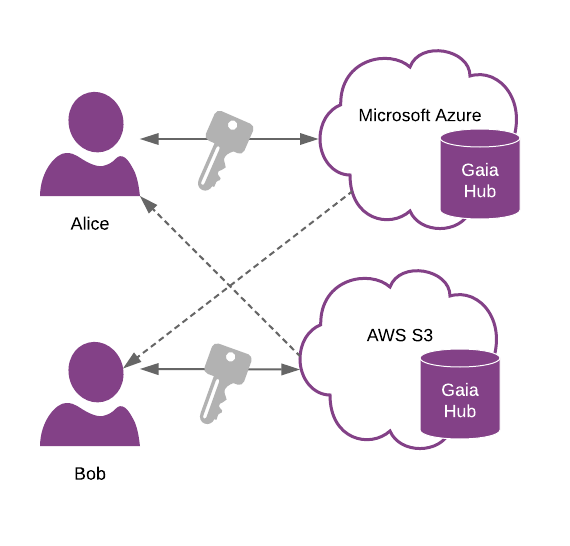
\includegraphics[width=200pt, height=200pt]{figures/gaia-storage}
			\caption{\label{fig:gaia-storage} How users interact with Gaia storage\protect\footnotemark}
		\end{figure}
		\footnotetext{\url{https://docs.blockstack.org/storage/overview.html}}
		
		Writing data to a Gaia hub involves a \texttt{POST} request along with a signed \textit{authentication} token. This token is signed by the private key which controls the particular bucket being written to. Separate buckets are used for each application, this ensures that a given private key grants access only to a specific bucket on the Gaia Server.
		
		\begin{figure}[h]
			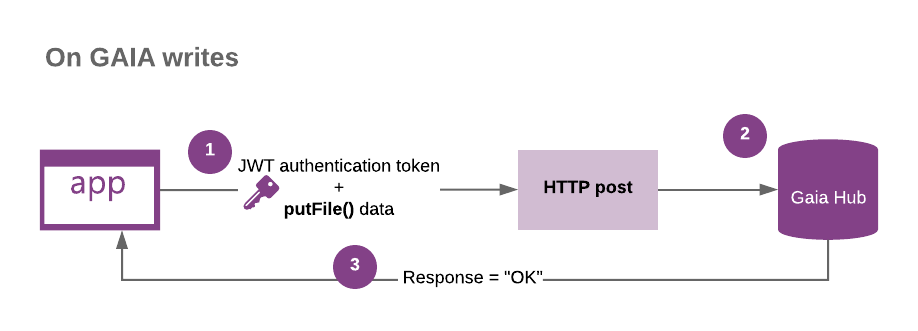
\includegraphics[width=\linewidth]{figures/gaia-writes}
			\caption{\label{fig:gaia-writes} The token ensures that a write is authorized\protect\footnotemark}
		\end{figure}
		\footnotetext{\url{https://docs.blockstack.org/storage/authentication.html}}
		
		Reading data from a user's Gaia hub involves a \textit{zonefile} lookup. This zonefile is a signed JSON object containing the URLs pointing to the user's Gaia data locker. Once verified that the zonefile is signed by user's key, a standard \texttt{HTTP} request is made to fetch the requested data.
		
		Figure~\ref{fig:gaia-overview} shows an overview of Gaia. Looking up data for a name works as follows:
		
		\begin{enumerate}
			\item Lookup the \textit{name} in the Virtualchain to get the (\textit{name, hash}) pair.
			\item Lookup the \textit{hash(name)} in Peer Network to get respective zonefile.
			\item Get the user's Gaia URL from the zonefile and lookup the URL to connect to storage backend.
			\item Fetch the requested data and verify the respective signature or hash.
		\end{enumerate}
		
		\begin{figure}[h]
			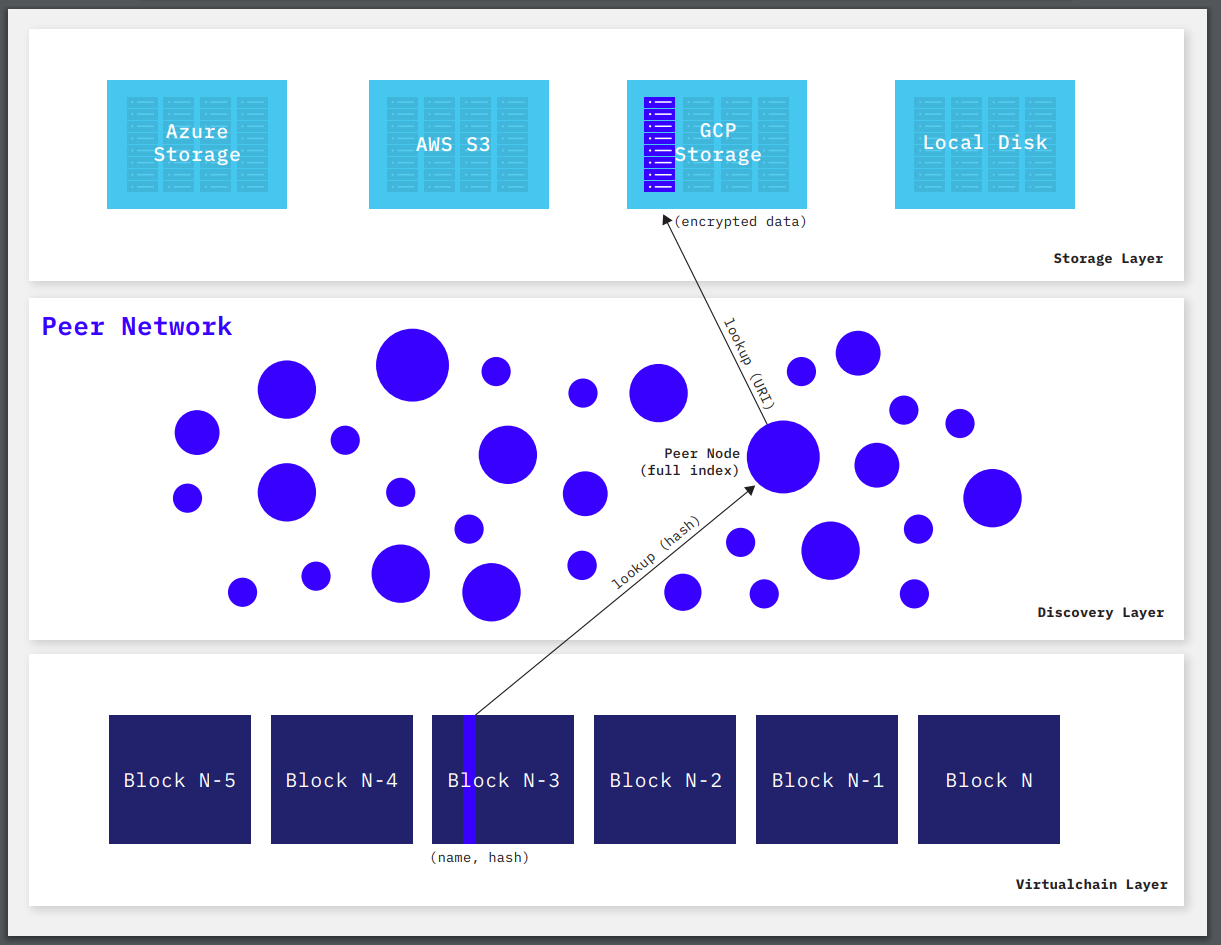
\includegraphics[width=\linewidth]{figures/gaia-overview}
			\caption{\label{fig:gaia-overview} Overview of Gaia and steps for looking up data.\protect\footnotemark}
		\end{figure}
		\footnotetext{\url{https://blockstack.org/whitepaper.pdf}}
		
	
\section{Identity}
	User identities are essential to using internet applications. In order to confirm their identity, users must provide some information. This information depends on the application's authentication process. If an application maintains a user database, it requires a username and a password and sometimes a second factor. If an application relies on a third-party, like Google\footnote{\url{https://developers.google.com/identity/}} or Facebook\footnote{\url{https://developers.facebook.com/docs/facebook-login/}} for identity management, it uses the OAuth 2.0 authentication\cite{hardt2012oauth} protocol, which identifies a user by generating an assertion from the identity service.
	
	Third party identity providers implementing the OAuth\footnote{\url{https://oauth.net/}} protocol often have their own version of implementation which leads to identity fragmentation across the web. OpenID\cite{recordon2006openid} is a decentralized identity protocol that allows users to create one identity which can be carried across multiple providers. However, the user still needs to trust one of the service providers with their identity information\cite{raval2016decentralized}.
	
	Another way of authenticating users with an application is by using digital certificates\cite{tycksen2001digital}. These certificates provide a proof of ownership of a public key. Authentication and management of public keys is facilitated using a Public Key Infrastructure (PKI)\cite{adams2003understanding} system. Currently, the most common approaches to PKIs are: Certificate Authorities (CAs) and PGP Web of Trust\cite{abdul1997pgp}. 
	
	A Certificate Authority (CA) acts a trusted third party responsible for management and distribution of digital certificates for a network of users\cite{fromknecht2014decentralized}. These trusted third parties introduces central control in a PKI system making them prone to single point of failure risk\cite{dooley2001designing}.
	
	In PGP Web of trust, authentication is entirely decentralized; users are able to designate others as trustworthy by signing their public keys. This process generates a digital certificate containing the user's public key and signatures from entities that have deemed him trustworthy. This system does benefit from its distributed nature as there is no central control. However, PGP does not offer identity retention. There is no guarantee of consistency and nothing prevents multiple users from creating public keys for the same identity\cite{fromknecht2014decentralized}.
	
	\subsection{Decentralized Public Key Infrastructure (DPKI)}
		\begin{figure}[h]
			\centering
			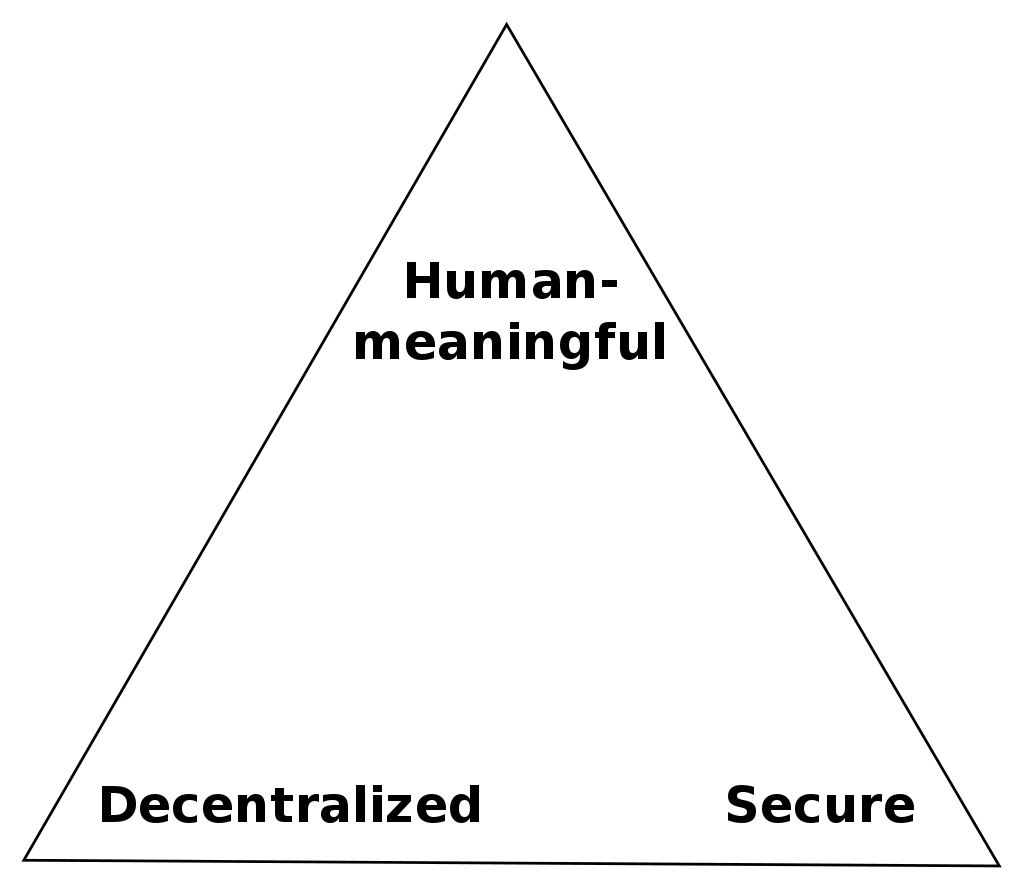
\includegraphics[width=200pt, height=150pt]{figures/zooko-triangle}
			\caption{\label{fig:zooko-triangle} Zooko's Triangle\protect\footnotemark}
		\end{figure}
		\footnotetext{\url{https://commons.wikimedia.org/wiki/File:Zooko\%27s_Triangle.svg}}
		
		The foundational precept of a DPKI is that \textit{identities belong to the entities they represent}. This requires designing a \textit{decentralized} infrastructure where every identity is controlled by its \textit{principal owner} and not by some trusted third party\cite{allen2015decentralized}.
		
		DPKI is essentially a system to gives unique names to participants in a network protocol. These names should have three desirable traits(Zooko's triangle) namely: \textit{Human-meaningful}, \textit{Decentralized} and \textit{Secure}. OpenID solved security and human-meaningfulness.
		
		Namecoin\footnote{\url{https://www.namecoin.org/}} was the first working solution that satisfied all three traits of Zooko's triangle by adding decentralization. It was the first fork of Bitcoin\cite{nakamoto2008bitcoin} protocol designed to act as a decentralized domain name server (DNS) for \textit{.bit} addresses. Namecoin's blockchain essentially could be used as an intermediary between a user and the service requesting user's identity\cite{raval2016decentralized}. It allowed a user to \textit{register} a name by creating a blockchain transaction. This transaction included the desired name which get embedded under the \textit{/id} namespace.
	
	\subsection{Decentralized Identifiers (DIDs)}
	A DID\footnote{\url{https://w3c-ccg.github.io/did-spec/}} is a new type of identifier that is globally unique, resolvable with high availability and cryptographically verifiable. DIDs typically contains cryptographic key pair which enables the controller of a DID to prove control over it.
	
	The concept of global unique decentralized identifiers is not new; Universally Unique Identifiers\footnote{\url{https://en.wikipedia.org/wiki/Universally_unique_identifier}}(UUIDs), also called Globally Unique Identifiers (GUIDs) were first such identifiers developed in 1980s and formally specified in RFC4122\footnote{\url{https://tools.ietf.org/html/rfc4122}}. Another class of identifiers knows as persistent identifiers was standardized as Uniform Resource Names (URNs) by RFC8141\footnote{\url{https://tools.ietf.org/html/rfc8141}}.
	
	However, UUIDs are not globally resolvable and URNs, if resolvable, require a central registry. Further, neither UUIDs or URNs have the ability to cryptographically verify ownership of the identifier. DIDs, on the other hand, fulfills all four requirements: persistence, global resolvability, cryptographically verifiability, and decentralization required for a self-sovereign identity\cite{smith2016identity}.
	
	\begin{figure}[h]
		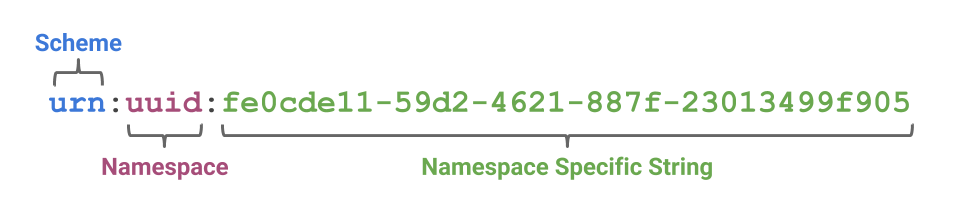
\includegraphics[width=\linewidth]{figures/urn-format}
		\caption{\label{fig:urn-format} The URN Specification}
	\end{figure}

	\begin{figure}[h]
		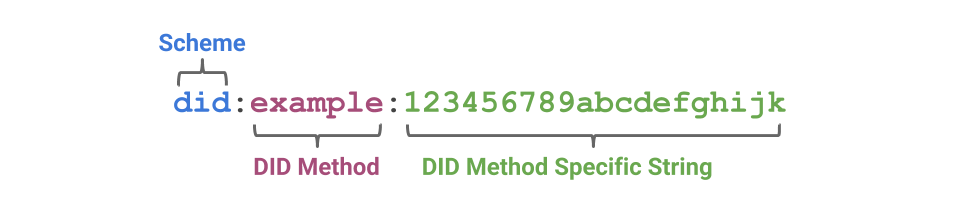
\includegraphics[width=\linewidth]{figures/did-format}
		\caption{\label{fig:did-format} The DID Specification}
	\end{figure}
	
	The DID (Figure~\ref{fig:did-format}\footnote{\url{https://w3c-ccg.github.io/did-primer/did-primer-diagrams/did-format.png}}) specification follows the same pattern as the URN (Figure~\ref{fig:urn-format}\footnote{\url{https://w3c-ccg.github.io/did-primer/did-primer-diagrams/urn-format.png}}) specification. The key difference is that with DIDs, the namespace component identifies a \textit{DID method} which defines how DIDs work with a specific blockchain. The \textit{DID method} specifications must define the format and generation of the method-specific identifier. The DID methods can also be developed for identifiers registered in federated or centralized identity management systems, thus creating a interoperability bridge between the worlds of centralized, federated and decentralized identifiers.
	
\section{Value}
	
\section{Computing}
	
\section{Bandwidth}